\begin{frame}{ChatGPT, l'IA générative de texte d'OpenAI}
\begin{block}{}
    \textbf{ChatGPT ?
    GPT (GPT3, GPT4, etc.)}\\

\begin{itemize}
    \item \textit{Generative Pre-trained Transformer}= modèle géant de prédiction de texte entraîné par OpenAI sur 500 milliards de mots (pour GPT3).
    \item Modèle encyclopédique
    \item Appartient à la famille des LLM= entraîné sur d'immenses quantités de données.
\end{itemize}
\end{block}
    
\begin{block}{}
\textbf{Chat (InstructGPT)}
    \begin{itemize}
        \item Une interface conversationnelle
        \item Fonctionne à partir des requêtes de l'usager : "le prompt"
    \end{itemize}
\end{block}
\end{frame}

\begin{frame}{Avec qui je "converse", lorsque j'échange avec ChatGPT ?
}
\textbf{1. Un agent conversationnel intégré à une interface au design conçu pour masquer la technique}
\vspace{5mm}
\begin{columns}[T,onlytextwidth]
\column{0.40\linewidth}
\small
\begin{itemize}
        \item le tout premier chatbot psychothérapeute (1966) conçu par Joseph Weizenbaum. Version Javascript par Michael Wallace et George Dunlop
    \end{itemize}
\column{0.50\linewidth}
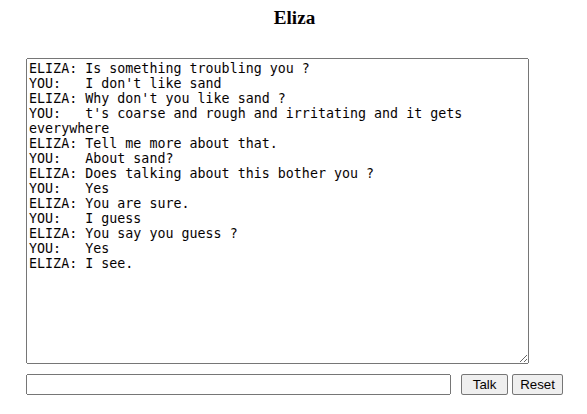
\includegraphics[width=0.80\textwidth]{04_Axe1_IAG/Images/Eliza.png}
\end{columns}
    
\end{frame}

\begin{frame}{Avec qui je "converse", lorsque j'échange avec ChatGPT ?}
    \textbf{2. Un LLM : un corpus de texte construit à partir du big data}

    \vspace{5mm}

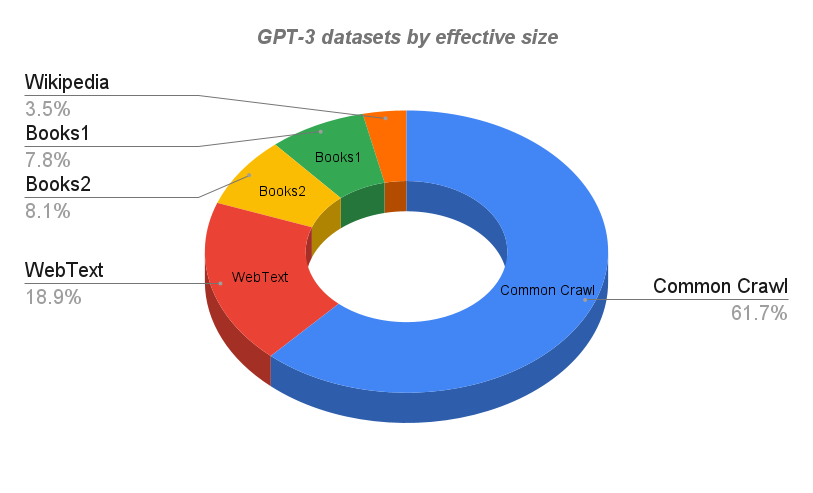
\includegraphics[width=0.80\textwidth]{04_Axe1_IAG/Images/2021-Alan-D-Thompson-GPT-3-datasets-by-effective-size-v2.png}
\end{frame}

\begin{frame}{Problématique des origines des données d'entraînement}
OpenAI ne publie pas la totalité des spécifications sur la construction de ses modèles.\\

Voici les trois catégories principales de données selon OpenAI :
\begin{itemize}
    \item \textbf{Données accessibles publiquement sur Internet}\\
    \textrightarrow{} Quid des données personnelles?
    \item \textbf{Données sous licence ou partenaires tiers}\\
    \textrightarrow{} Contenu auquel OpenAI a légalement accès
    \item Données fournies ou générées avec participation humaine\\
    \textrightarrow{} Données annotées, modèles entraînés, fine-tuning. digital labour.
\end{itemize}

Question de la neutralité des llm.
\end{frame}

\begin{frame}{Les biais de l'IA et des algorithmes}
    \textbf{Biais de l'IA =} Désignent les systèmes d’IA qui produisent des résultats biaisés répétant les préjugés humains au sein d’une société\\

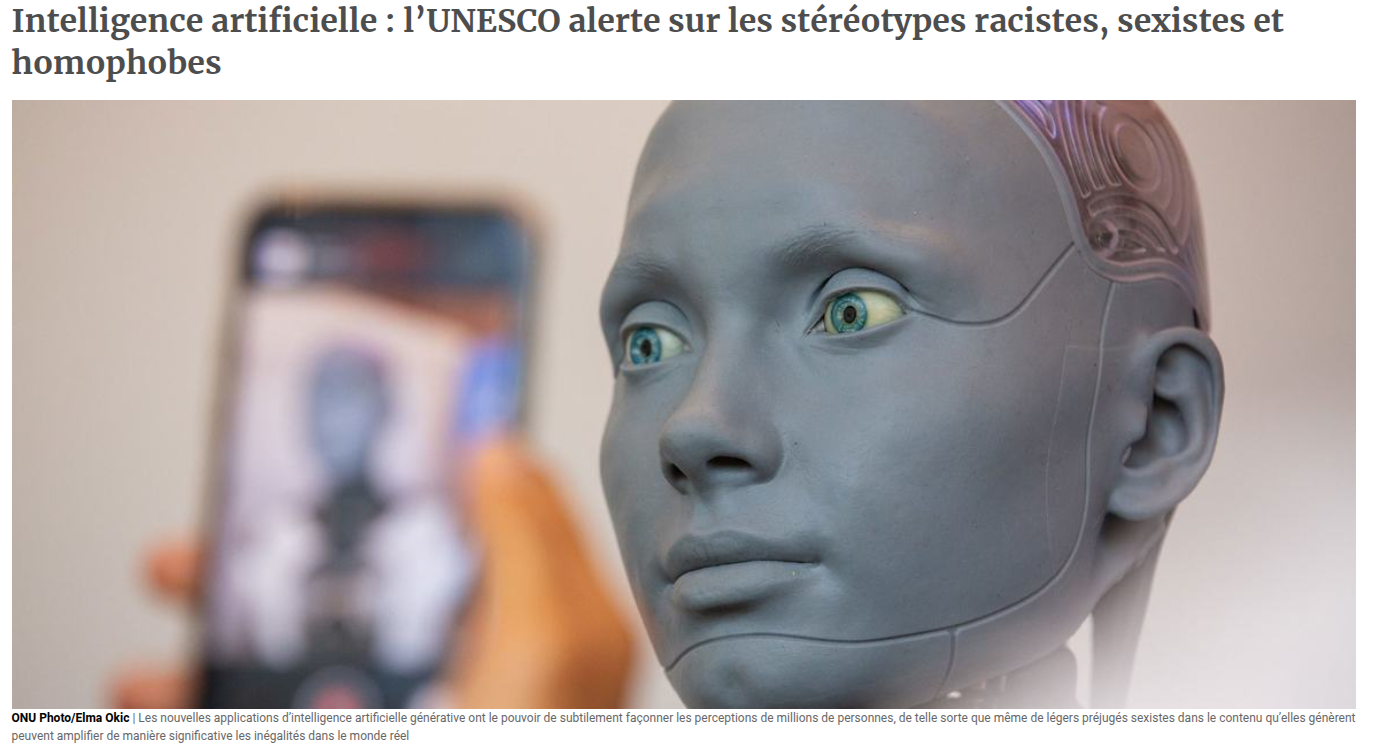
\includegraphics[width=0.60\textwidth]{04_Axe1_IAG/Images/UNESCO.png}

\end{frame}

\begin{frame}{ChatGPT et les biais de genre}

Isabelle Collet, professeure en sciences de l’éducation à l’Université de Genève et spécialiste des questions de genre dans le numérique, dans son livre \textit{Le numérique est l’affaire de toutes} distingue trois principaux risques :
\begin{itemize}
    \item \textbf{L’apprentissage des stéréotypes}. Ex de Wikipédia.
    \item \textbf{La discrimination dans l’aide à la décision}. Renforcement des inégalités déjà présentes dans la société, par exemple en matière d’embauche, de rémunération, de promotion, d’octroi de prêts ou encore d’orientation scolaire.
    \item \textbf{Le manque de diversité dans les métiers du numérique.} Invisibilisation d'une partie des besoins et des expériences de la population.
\end{itemize}
\end{frame}

\begin{frame}{Midjourney et les stéréotypes racistes}
\begin{columns}[T,onlytextwidth]
\column{0.50\linewidth}

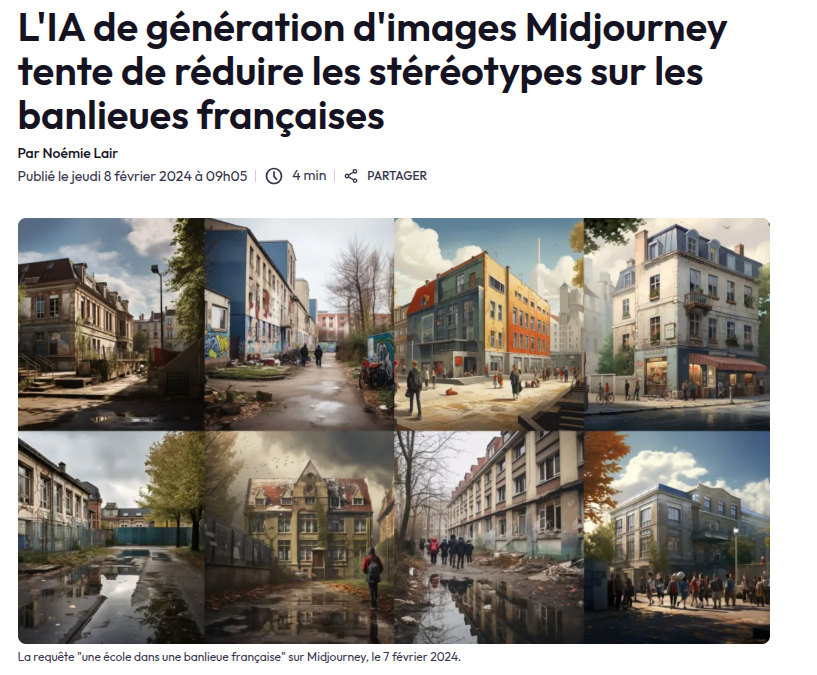
\includegraphics[width=0.80\textwidth]{04_Axe1_IAG/Images/franceinter.png}\\
\small
\href{https://www.radiofrance.fr/franceinter/tags-dechets-batiments-delabres-quand-l-ia-reproduit-les-stereotypes-sur-les-banlieues-3334839}{Podcast sur France Inter}.
\column{0.50\linewidth}

\includegraphics[width=0.90\textwidth]{04_Axe1_IAG/Images/refecltions_before_storm.png}\\
\small
Alenichev, Arsenii et al., \href{https://www.thelancet.com/journals/langlo/article/PIIS2214-109X(23)00329-7/fulltext?utm_source=generationia.flint.media&utm_medium=referral&utm_campaign=dall-e-midjourney-les-stereotypes-raciaux-sont-encore-tenaces-dans-l-ia}{\textit{Reflections before the storm: the AI reproduction of biased imagery in global health visuals}}, 2023

\end{columns}
\end{frame}

\begin{frame}{Quid du coût écologique?}

Ce qu'il faut pour entraîner des modèles d'IAG:
\begin{itemize}
\item Construire des serveurs
    \item De l'eau pour refroidir les serveurs
    \item De l'électricité
\end{itemize}
\begin{block}
\centering
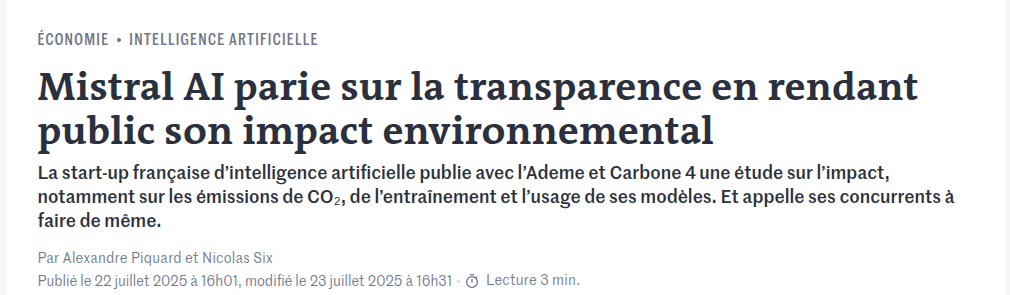
\includegraphics[width=0.60\textwidth]{04_Axe1_IAG/Images/mistral_ecolo.png}    
\end{block}


Pour l'entraînement de Mistral Large 2, après 18 mois d'utilisation:
\begin{itemize}
    \item 20,4 ktCO₂e
\item 281 000 m3 d'eau consommée
\item 660 kg Sb eq (unité standard pour l'épuisement des ressources).
\end{itemize}

\end{frame}

\begin{frame}{Pourquoi ChatGPT n'est PAS un moteur de recherche ?}
    
ChatGPT n’a aucune compréhension de votre question ni même de sa réponse, qui résulte d'un calcul statistique croisant le contexte de votre requête et les différentes données qu’il a à sa disposition.
\end{frame}

\begin{frame}{Attention aux hallucinations!}
    \textbf{Exemple: invention d'une source bibliographique.}\\
    \vspace{5mm}
    \centering
    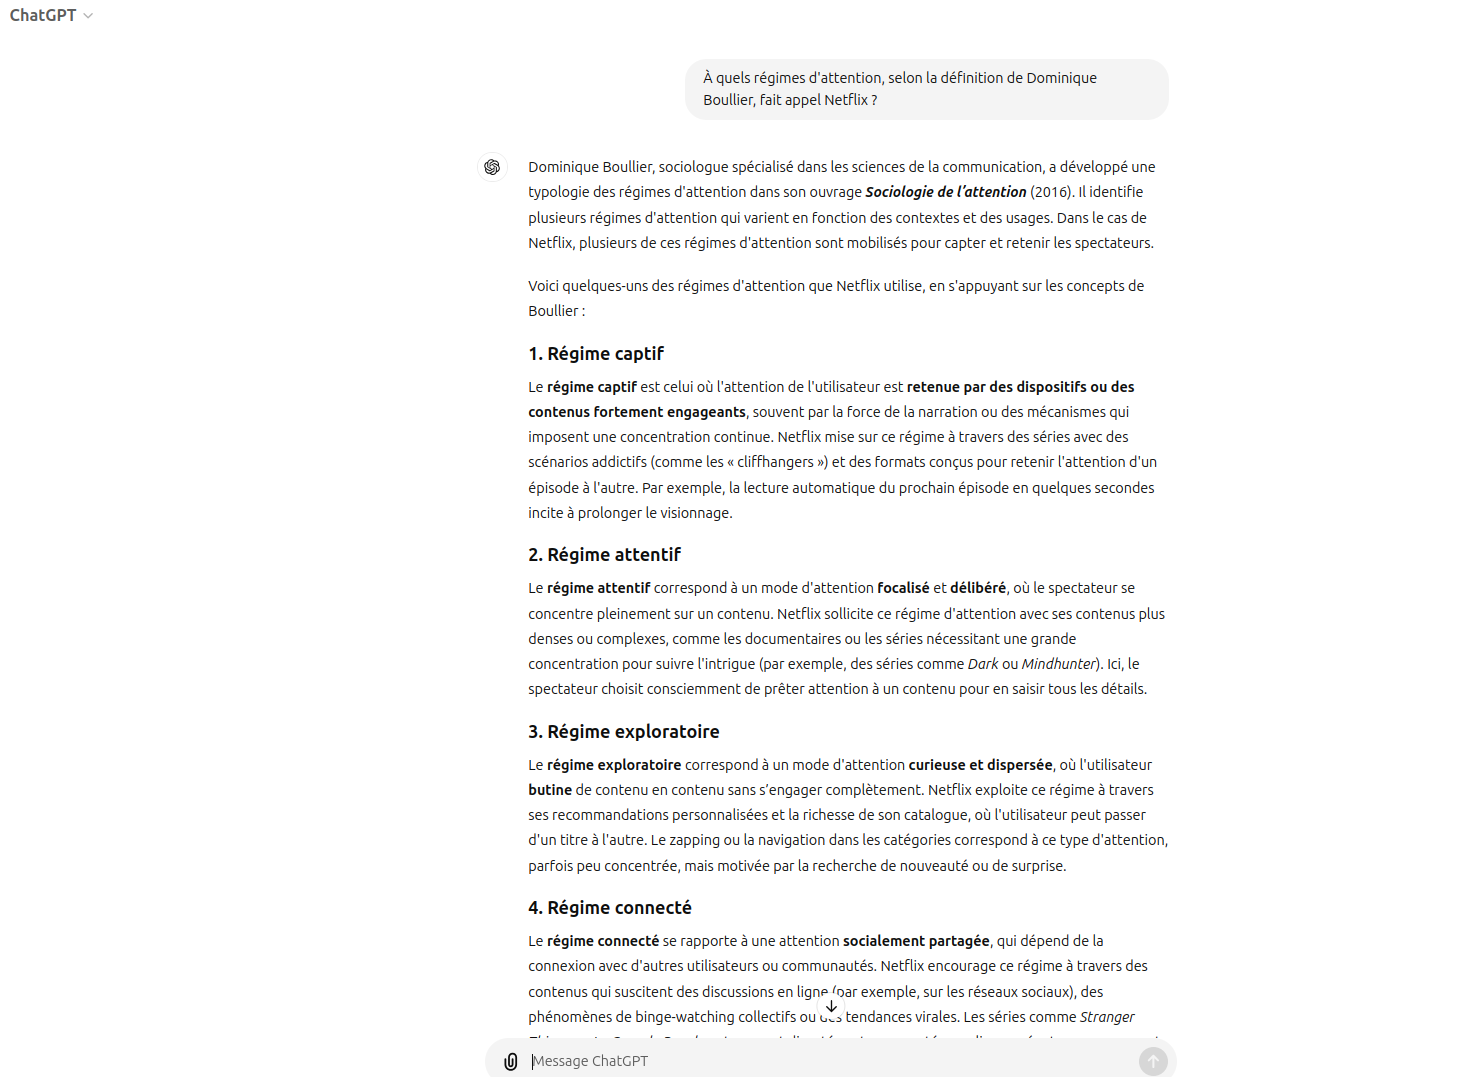
\includegraphics[width=0.70\textwidth]{04_Axe1_IAG/Images/gptHalluBoullier.png}
\end{frame}

\begin{frame}{ChatGPT search, un moteur de réponse}
\begin{itemize}
    \item Un service qui nous propose une synthèse de certaines sources en fonction de notre requête
    \item Une liste de sources (critères de sélection non précisés)
    \item Pas de rémunération des sources
    \item Une logique de plus en plus prescriptive
    \item Quid de la compétence d'évaluation et d'esprit critique ?
\end{itemize}
    
\end{frame}

\begin{frame}{Les IAG dans le secteur des industries culturelles et créatives : une communauté divisée}
\begin{itemize}
    \item Les modèles entraînés respectent-ils le droit d'auteur?
    \item L'IA est-elle un outil de création comme un autre, ou sert-elle une imposture ?
    \item En améliorant la productivité, dans quelle mesure les IAG menacent-elle les professionnels ?
    \item Le recours à l'IAG vaut-il vraiment le coup (engagement : enjeux éthiques et écologiques) ?
\end{itemize}

\end{frame}